\begin{figure*}[t]
\centering
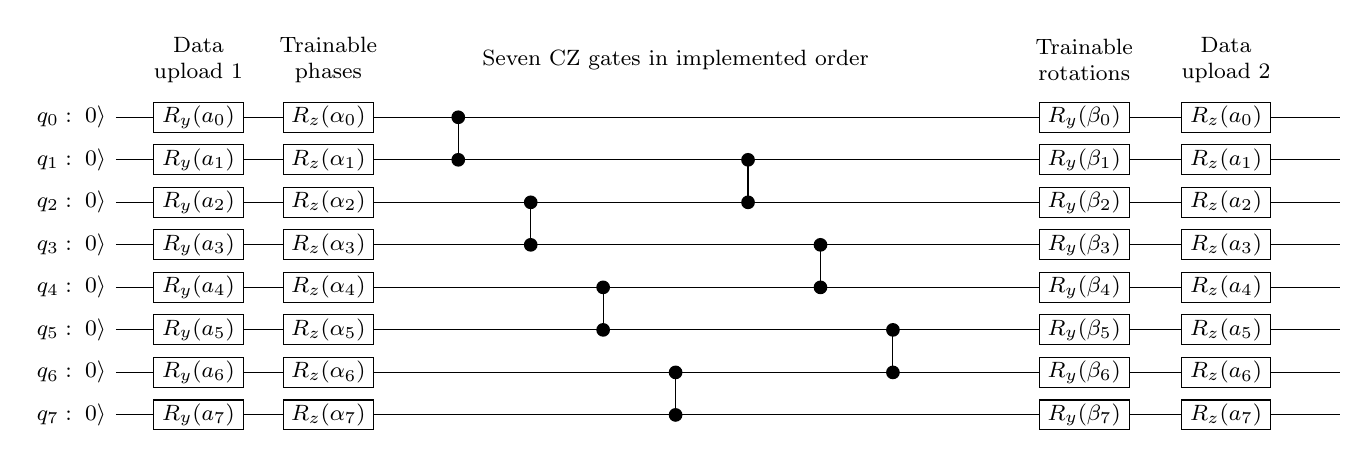
\begin{tikzpicture}[x=1cm,y=0.54cm,gate/.style={draw,fill=white,minimum width=1.14cm,minimum height=0.38cm,inner sep=1pt,font=\footnotesize},dot/.style={circle,fill,inner sep=1.75pt}]
\draw (0,0) -- (15.55,0);
\node[left,font=\footnotesize] at (0,0) {$q_0:\;\lvert0\rangle$};
\node[gate] at (1.05,0) {$R_y(a_0)$};
\node[gate] at (2.7,0) {$R_z(\alpha_0)$};
\node[gate] at (12.30,0) {$R_y(\beta_0)$};
\node[gate] at (14.10,0) {$R_z(a_0)$};
\draw (0,-1) -- (15.55,-1);
\node[left,font=\footnotesize] at (0,-1) {$q_1:\;\lvert0\rangle$};
\node[gate] at (1.05,-1) {$R_y(a_1)$};
\node[gate] at (2.7,-1) {$R_z(\alpha_1)$};
\node[gate] at (12.30,-1) {$R_y(\beta_1)$};
\node[gate] at (14.10,-1) {$R_z(a_1)$};
\draw (0,-2) -- (15.55,-2);
\node[left,font=\footnotesize] at (0,-2) {$q_2:\;\lvert0\rangle$};
\node[gate] at (1.05,-2) {$R_y(a_2)$};
\node[gate] at (2.7,-2) {$R_z(\alpha_2)$};
\node[gate] at (12.30,-2) {$R_y(\beta_2)$};
\node[gate] at (14.10,-2) {$R_z(a_2)$};
\draw (0,-3) -- (15.55,-3);
\node[left,font=\footnotesize] at (0,-3) {$q_3:\;\lvert0\rangle$};
\node[gate] at (1.05,-3) {$R_y(a_3)$};
\node[gate] at (2.7,-3) {$R_z(\alpha_3)$};
\node[gate] at (12.30,-3) {$R_y(\beta_3)$};
\node[gate] at (14.10,-3) {$R_z(a_3)$};
\draw (0,-4) -- (15.55,-4);
\node[left,font=\footnotesize] at (0,-4) {$q_4:\;\lvert0\rangle$};
\node[gate] at (1.05,-4) {$R_y(a_4)$};
\node[gate] at (2.7,-4) {$R_z(\alpha_4)$};
\node[gate] at (12.30,-4) {$R_y(\beta_4)$};
\node[gate] at (14.10,-4) {$R_z(a_4)$};
\draw (0,-5) -- (15.55,-5);
\node[left,font=\footnotesize] at (0,-5) {$q_5:\;\lvert0\rangle$};
\node[gate] at (1.05,-5) {$R_y(a_5)$};
\node[gate] at (2.7,-5) {$R_z(\alpha_5)$};
\node[gate] at (12.30,-5) {$R_y(\beta_5)$};
\node[gate] at (14.10,-5) {$R_z(a_5)$};
\draw (0,-6) -- (15.55,-6);
\node[left,font=\footnotesize] at (0,-6) {$q_6:\;\lvert0\rangle$};
\node[gate] at (1.05,-6) {$R_y(a_6)$};
\node[gate] at (2.7,-6) {$R_z(\alpha_6)$};
\node[gate] at (12.30,-6) {$R_y(\beta_6)$};
\node[gate] at (14.10,-6) {$R_z(a_6)$};
\draw (0,-7) -- (15.55,-7);
\node[left,font=\footnotesize] at (0,-7) {$q_7:\;\lvert0\rangle$};
\node[gate] at (1.05,-7) {$R_y(a_7)$};
\node[gate] at (2.7,-7) {$R_z(\alpha_7)$};
\node[gate] at (12.30,-7) {$R_y(\beta_7)$};
\node[gate] at (14.10,-7) {$R_z(a_7)$};
\draw (4.35,0) -- (4.35,-1);
\node[dot] at (4.35,0) {};
\node[dot] at (4.35,-1) {};
\draw (5.27,-2) -- (5.27,-3);
\node[dot] at (5.27,-2) {};
\node[dot] at (5.27,-3) {};
\draw (6.19,-4) -- (6.19,-5);
\node[dot] at (6.19,-4) {};
\node[dot] at (6.19,-5) {};
\draw (7.11,-6) -- (7.11,-7);
\node[dot] at (7.11,-6) {};
\node[dot] at (7.11,-7) {};
\draw (8.03,-1) -- (8.03,-2);
\node[dot] at (8.03,-1) {};
\node[dot] at (8.03,-2) {};
\draw (8.95,-3) -- (8.95,-4);
\node[dot] at (8.95,-3) {};
\node[dot] at (8.95,-4) {};
\draw (9.87,-5) -- (9.87,-6);
\node[dot] at (9.87,-5) {};
\node[dot] at (9.87,-6) {};
\node[font=\footnotesize,align=center] at (1.05,1.35) {Data\\upload 1};
\node[font=\footnotesize,align=center] at (2.7,1.35) {Trainable\\phases};
\node[font=\footnotesize] at (7.11,1.35) {Seven CZ gates in implemented order};
\node[font=\footnotesize,align=center] at (12.30,1.35) {Trainable\\rotations};
\node[font=\footnotesize,align=center] at (14.10,1.35) {Data\\upload 2};
\end{tikzpicture}
\caption{Protected TQK8 state-preparation circuit, read from left to right. Here $a_q$ is an encoded feature, $\alpha_q=\theta_q$, and $\beta_q=\theta_{8+q}$. A line with two filled endpoints denotes CZ. The seven gates are drawn sequentially to preserve the source order; no hardware schedule or transpiled depth is implied. The circuit has no measurement in exact-state evaluation.}
\label{fig:tqk8-circuit}
\end{figure*}
